\documentclass[a4paper,twocolumn,5p]{elsarticle}

\usepackage{hyperref}
%\usepackage{lineno}
%\modulolinenumbers[5]

\usepackage{booktabs}
\usepackage{graphicx}
\usepackage{xspace}
\usepackage{booktabs}
\usepackage[draft]{fixme}

\journal{Environment International}

%% `Elsevier LaTeX' style
\bibliographystyle{elsarticle-num}
%%%%%%%%%%%%%%%%%%%%%%%

\begin{document}

% Macro para escribir NO$_2$
\newcommand{\no}{NO\textsubscript{2}\xspace}

\begin{frontmatter}

\title{A comparison of probabilistic forecasting methods for extreme \no pollution episodes}

\author{Sebasti\'an P\'erez Vasseur}
\address{Artificial Intelligence Department\\Universidad Nacional de
  Educaci\'on a Distancia --- UNED\\c/ Juan del Rosal, 16, Madrid, Spain}

\author{Jos\'e L. Aznarte\fnref{myfootnote}}
\address{Artificial Intelligence Department\\Universidad Nacional de
  Educaci\'on a Distancia --- UNED\\c/ Juan del Rosal, 16, Madrid, Spain}
\ead{jlaznarte@dia.uned.es}

\fntext[myfootnote]{This work has been partially funded by Ministerio
  de Econom\'ia y Competitividad, Gobierno de Espa\~na, through a
  \emph{Ram\'on y Cajal} grant % awarded to Dr Aznarte
  (reference: RYC-2012-11984).}


\begin{abstract}

\end{abstract}

\begin{keyword}
probabilistic forecasting \sep air quality \sep quantile regression
\sep nitrogen dioxide \sep Madrid
\end{keyword}

\end{frontmatter}

%\linenumbers

\section{Introduction}
\label{sec:intro}



\section{Probabilistic forecasting with quantile regression}
\label{sec:probForec}

As mentioned above, the prediction from most regression models is a
point estimate of the conditional mean of a dependent variable, or
response, given a set of independent variables or predictors. However,
the conditional mean measures only the center of the conditional
distribution of the response, and if we need a more complete summary
of this distribution, for example in order to estimate the associated
uncertainty, quantiles are in order. The 0.5 quantile (i.e., the
median) can serve as a measure of the center, and the 0.9 quantile
marks the value of the response below which reside the 90\% of the
predicted points. Recent advances in computing have inducted the
development of regression models for predicting given quantiles of the
conditional distribution. The technique is called quantile regression
(QR) and was first proposed by Koenker in 1978
\cite{koenker_regression_1978} based on the intuitions of the
astronomer and polymath Rudjer Boscovich in the 18th
century. Elaborating from the same concept of estimating conditional
quantiles from different perspectives, several statistical and CI
models that implement this technique have been developed: from the
original linear proposal to multiple or additive regression, neural
networks, support vector machines, random forests etc.

Quantile regression has gained an increasing attention from very
different scientific disciplines \cite{yu_quantile_2003}, including
financial and economic applications \cite{fitzenberger_economic_2002},
medical applications \cite{soyiri_forecasting_2012}, wind power
forecasting \cite{zhang_review_2014}, electric load forecasting
\cite{7423794,gibbons_quantile_2014}, environmental modelling
\cite{cade_gentle_2003} and meteorological modelling
\cite{bjornar_bremnes_probabilistic_2004} (these references are just
examples and the list is not exhaustive). To our knowledge, despite
its success in other areas, quantile regression has not been applied
in the framework of air quality% , with the exception of
% \cite{martinez-silva_forecasting_2016}
.

Thus, as we can estimate an arbitrary quantile and forecast its
values, we can also estimate the full conditional distribution, which
will entail us to the results presented in Section \ref{sec:results}.

Also, probabilistic forecasting is an advantage as we need to predict 
when the target will be above a certain threshold (180). So instead of having a 
Yes/No Answer, we are calculating the probability of the target being the above 
the threshold.

Among the array of methods that allow to estimate and forecast
data-driven conditional quantiles, in this study we have chosen
k-neighbors quantile regression, quantile regression forests and quantile XGBoost. 
We will compare the different algorithms through the CRPS metric for the 
distribution and the RMSE, MAE, Correlation and Bias for the quantile 50.

\section{Data description and experimental design}

\subsection{Training Data}

There are 20 pollution stations around the city and they are organized in different
zones as you can see in the picture below:

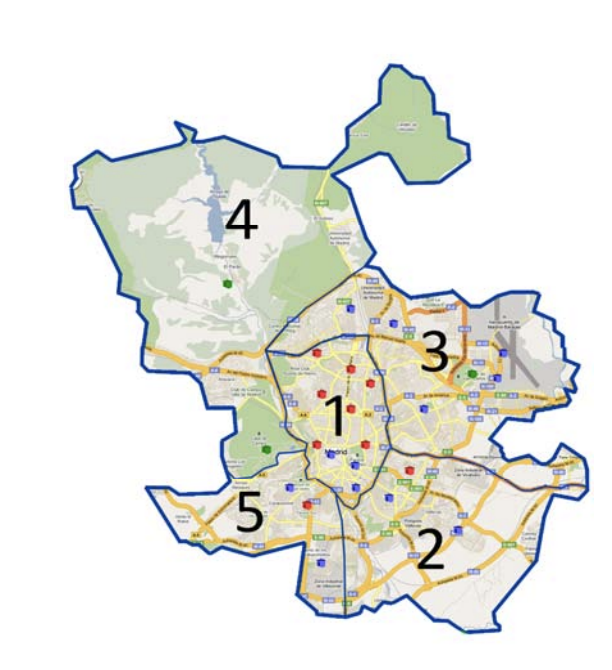
\includegraphics[width=0.4\textwidth]{zonas_madrid}


In 20 pollution stations in Madrid, we have an almost complete hourly record of the last 5 years of:
\begin{itemize}
  \item the levels of NO2 and O3
  \item calendar variables that represent the status of the day: bank holiday, laboral, type of holiday ...
  \item weather data: Precipitation, Temperature, Humidity, Wind
  \item ECMWF numerical pollution prediction
\end{itemize} 

\subsection{Feature Preprocessing}

\subsubsection{Calendar Fields Summary}

We will create 2 variables: one which indicates the day has a positive effect on pollution and 
another one for negative effect. We use a linear regression to predict the NO2 value only from the calendar variables.
As we can see in the chart, some variables have a positive effect and others a negative effect, based on the
sign of the coefficient applied to that feature:

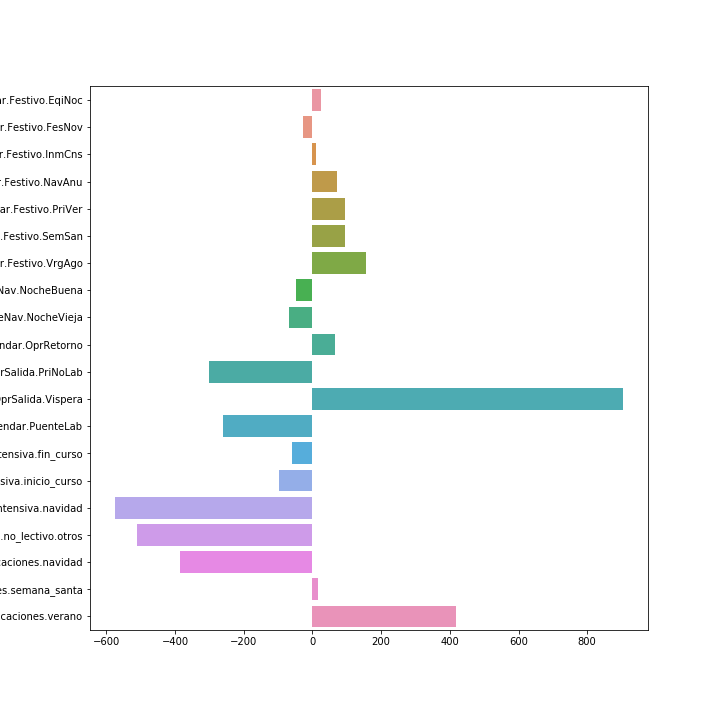
\includegraphics[width=0.4\textwidth]{calweights}

Then we create the 2 new variables as the sum of the positive features and the sum of the negative features respectively.

\subsubsection{Seasonality Extraction}

We extract the 6 main factors from the Fourier Transform of the signal. The chart displays the absolute value of
the Fourier components of the time series:

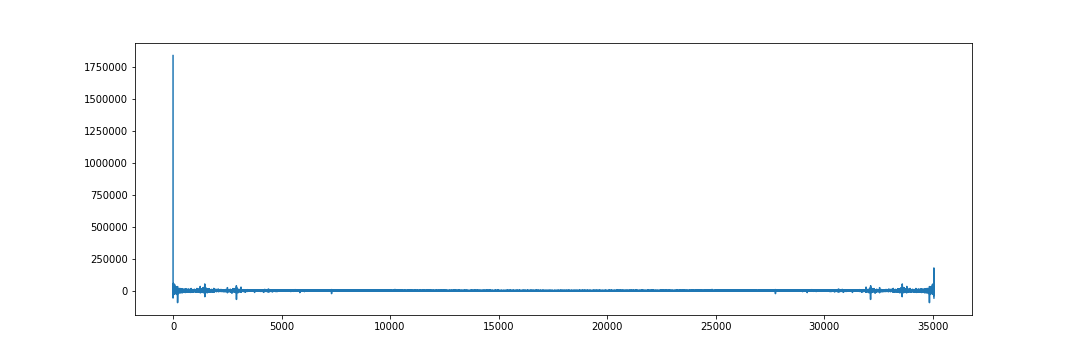
\includegraphics[width=0.4\textwidth]{decomposition}

If we zoom on the first 3000 components:

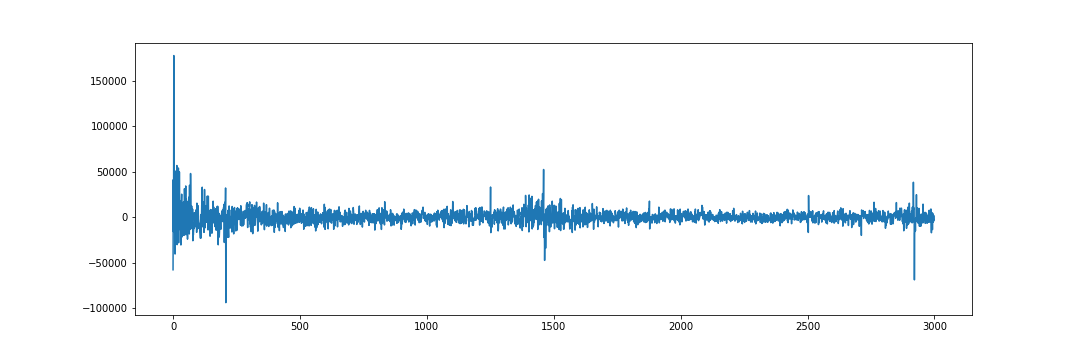
\includegraphics[width=0.4\textwidth]{decompositionzoom}

As we can see there are some dominant frequencies that show the time series has a strong seasonality. The 5 main 
frequencies are:

\begin{itemize}
  \item Every 12 hour Seasonality
  \item Yearly Seasonality
  \item Daily Seasonality
  \item Every 4 year seasonality
  \item Weekly Seasonality
\end{itemize} 

Therefore, we will create as input the output of periodic functions (cos) whose frequency is equal to the ones found 
above. This will enable the machine learning model learn the seasonality of our time series.

\subsubsection{Previous Values}

As with any forecast technique based on machine learning, we add previous values to improve the accuracy 
of the analysis. Based on the seasonal analysis, we see it's interesting to add a week of values. We will not 
add more to keep a reasonable number of features as input.

\subsection{k-Neighbors}

The probabilistic k-Neighbors is based on the competition entry from 
[K-nearest neighbors for GEFCom2014 probabilistic wind power forecasting]. 
This algorithm is based on the standard k-Neighbor, where instead of aggregating the targets of the
k nearest points to the input (by taking the mean or median for example), it builds a distribution 
from those neighbors.

We need to find an optimal number k for our model. We will use the CRPS of the predicted distribution
to get the best k. As you can see in the chart, 50 seems to be the optimal 
number of neighbor.

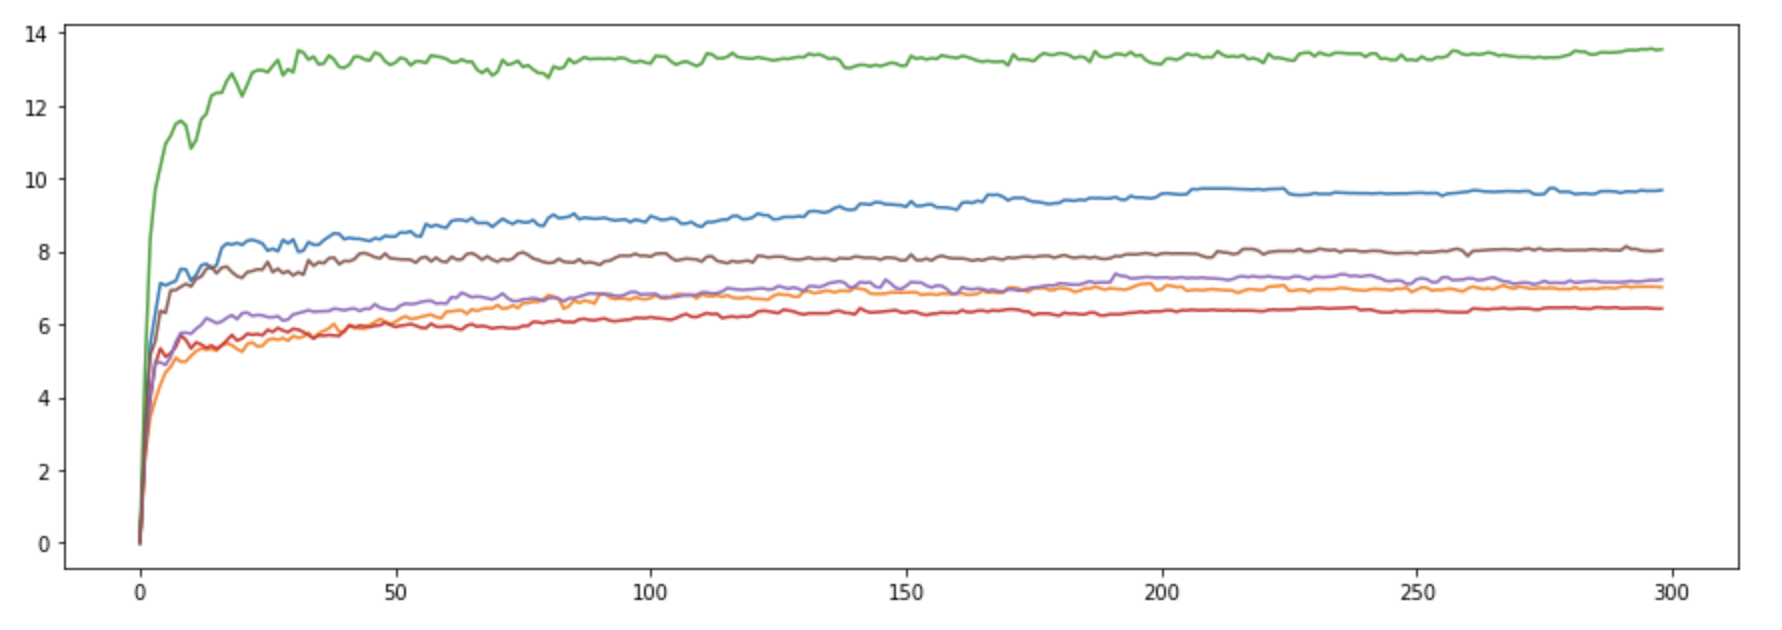
\includegraphics[width=0.4\textwidth]{kneighbor_crps}

\subsection{Quantile Random Forest}

We will use the quantile random forest as described in \cite{randomforestdesc}. Quantiles are built 
from the observations in the training set. We take the observation points that belong to the 
same leaf than the input and we build a distribution from those points. See figure for explanation:

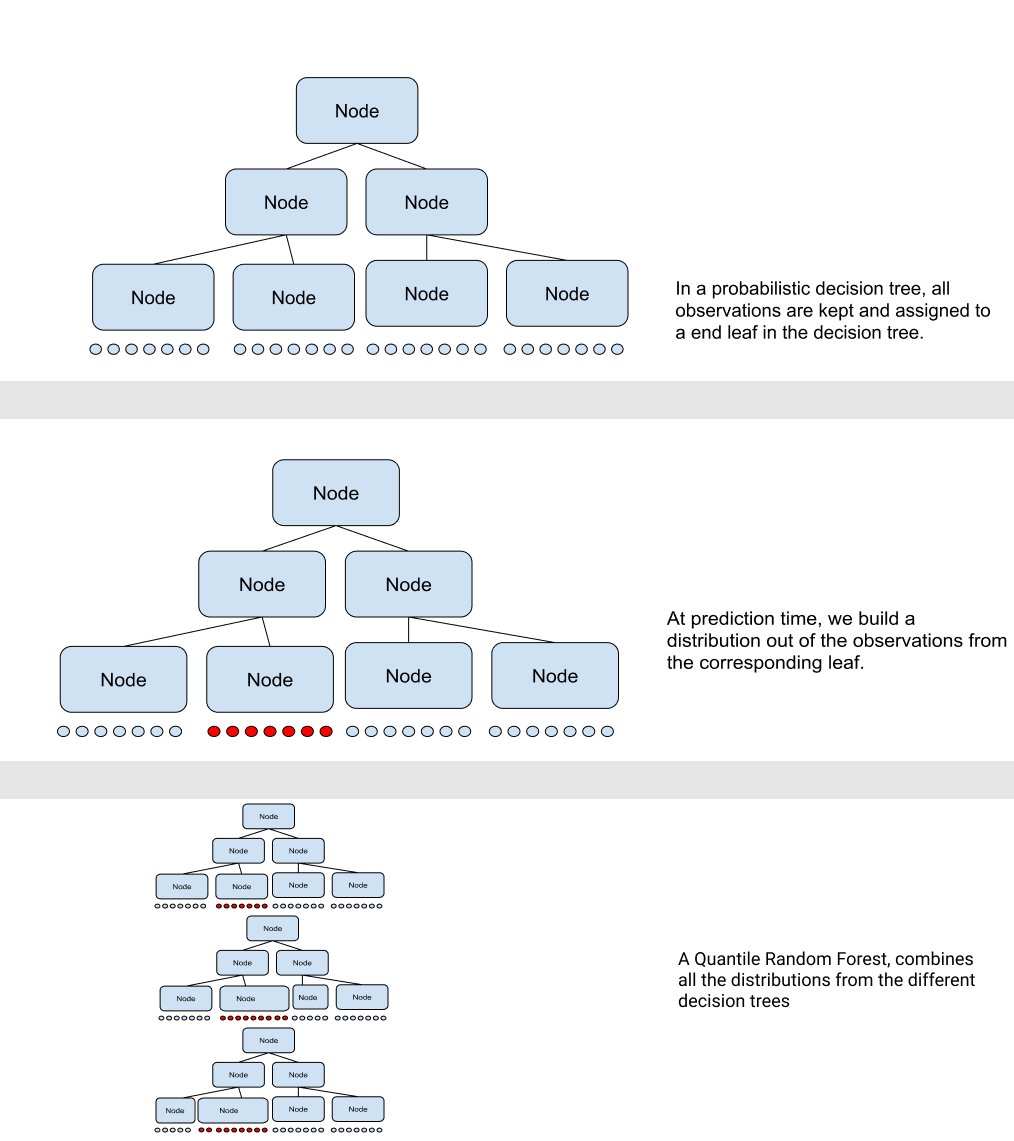
\includegraphics[width=0.4\textwidth]{quantile_random_forest}

For a detailed discussion on quantile regression forests, see
\cite{meinshausen_quantile_2006}.

\subsection{Gradient Boosted Tree}

Gradient Boosted Trees is a technique that consist on growing trees based on the compromise 
of a cost function and a regularization functions. This cost function is usually used to forecast 
the mean of the signal. But we are modifying the cost function 
in order to forecast the quantile of the function. 

s an illustration of the concept (for a detailed discussion of 
quantile regression, refer to \cite{koenker_quantile_2005}), given a 
set of vectors $(x_i, y_i)$, in point forecasting we are usually 
interested in what prediction $\hat y(x) = \alpha_0 + \alpha_1 x$
minimizes the mean squared error,
\begin{equation}
  \label{eq:1}
  E = \frac{1}{n} \sum^n_i \epsilon_i =
  \frac{1}{n} \sum^n_i [ y_i - (\alpha_0 + \alpha_1 x) ]^2.
\end{equation}
This prediction is the conditional sample mean of $y$ given $x$% , that
% is, $\hat y(x) = \hat\alpha_0 + \hat\alpha_1 x$
, or the location of the conditional distribution. But we could be
interested in estimating the conditional median (i.e., the 0.5
quantile) instead of the mean, in which case we should find the
prediction $\hat y(x)$ which minimizes the mean absolute error,
\begin{equation}
  \label{eq:2}
  E = \frac{1}{n} \sum^n_i \epsilon_i =
  \frac{1}{n} \sum^n_i | y_i - (\alpha_0 + \alpha_1 x) |.
\end{equation}
The fact is that, apart from the 0.5 quantile, it is possible to
estimate any other given quantile $\tau$. In that case, instead of
(\ref{eq:2}), we could minimize
\begin{equation}
  \label{eq:3}
E= \frac{1}{n} \sum^n_i f( y_i - (\alpha_0 + \alpha_1 x))
\end{equation}
where
\begin{equation}
  \label{eq:4}
  f(y-q) = \left\{ 
\begin{array}{l l}
\tau (y-q) & \quad \mbox{if $y \ge q$}\\
(1-\tau) (q-y) & \quad \mbox{if $y < q$}\\
\end{array} \right.,
\end{equation}
with $\tau \in (0,1)$. Equation (\ref{eq:3}) represents the
median when $\tau=0.5$ and the $\tau$-th quantile in any other case.

By forecasting different quantiles, we
can forecast the CDF of the time series. 
The main drawback is that we need to build a model per quantile. And since quantiles are calculated separately, 
we can have quantile crossing, i.e. the non monotonicity of the predicted CDF. 

In order to solve that, we will apply the technique from . This chart shows the predicted 10 and 90 
percentiles of the first 100 values.

\label{sec:mm}

\subsection{Protocol for high \no concentration episodes}
\label{sec:madr-prot-high}


\subsection{Nitrogen dioxide data}
\label{sec:no2}


\subsection{Weather data}
\label{sec:weather-data}

\subsection{ECMWF numerical pollution prediction}
\label{sec:ecmwf-numer-poll}

The European Centre for Medium-Range Weather Forecasts implements the Copernicus Atmosphere Monitoring Service.
This service provides CAMS delivers a saily production of near-real-time European air quality analyses and forecasts 
with a multi-model ensemble system. 
As you can see in the picture, the scope of the forecast is european and does not have the needed granularity to forecast 
the levels of NO2 in a station.


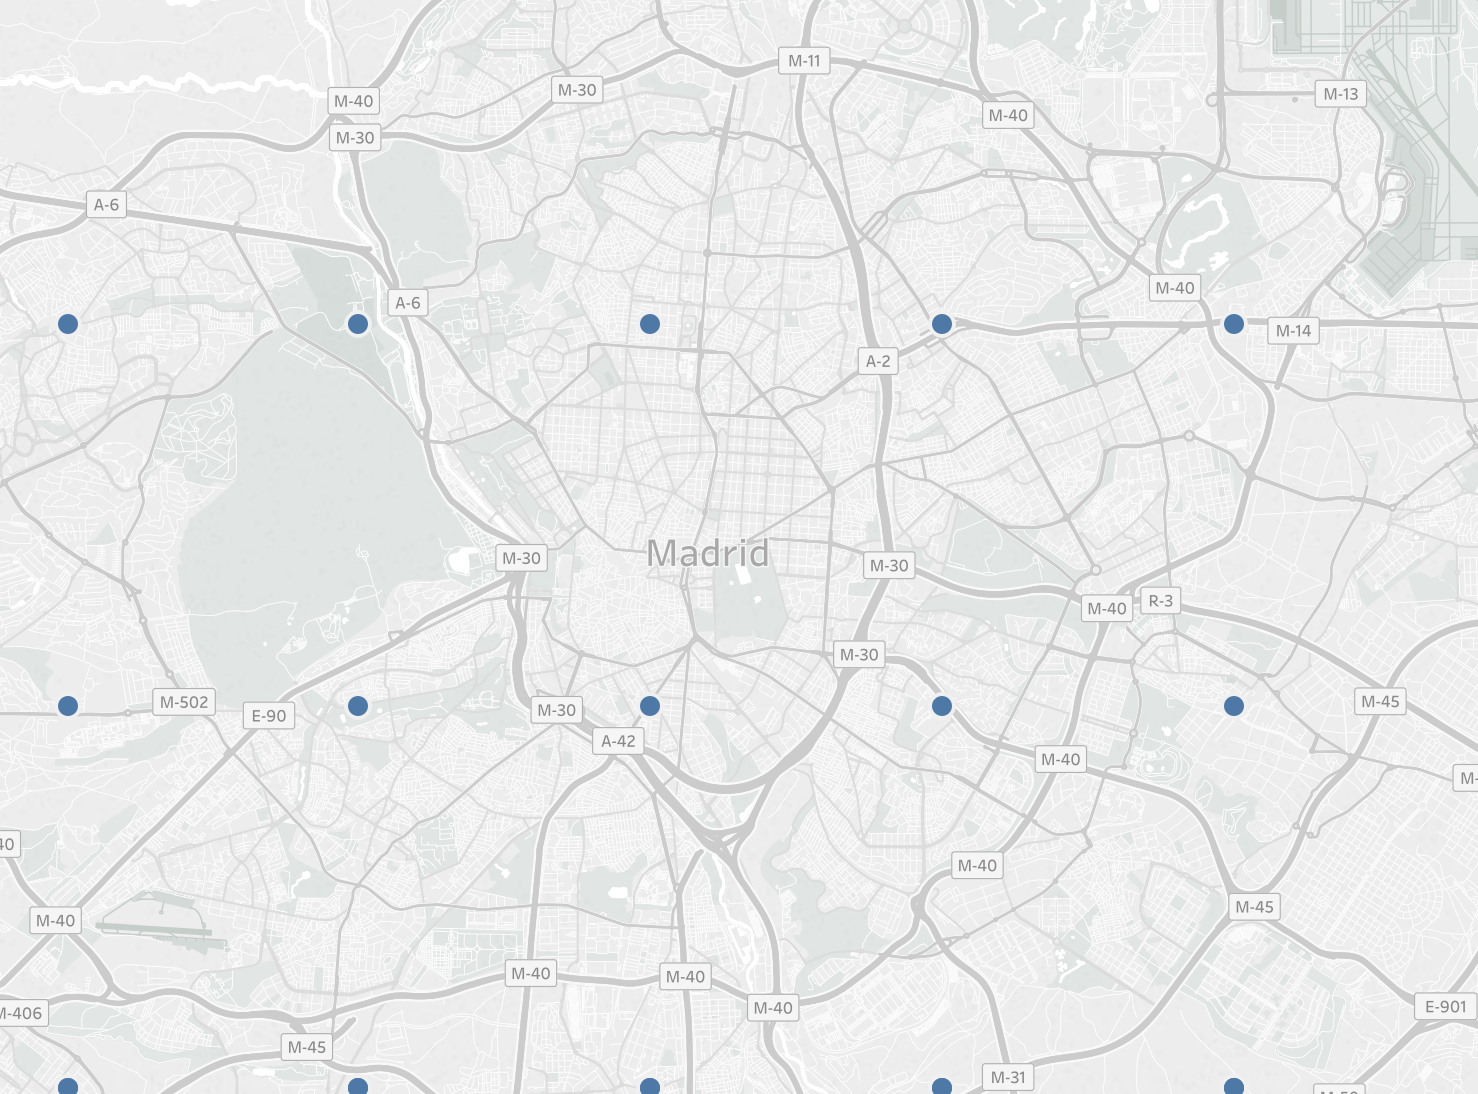
\includegraphics[width=0.4\textwidth]{camspoints}

\subsection{Experimental design}
\label{sec:experimental-design}

We will train the models with data prior to 2017 and we will test our models with 2017 data. We will always test with 
predictions done at 10:00, as this is the time the forecast will be done and the alert will be decided or not.

Also, we will create different models for each horizon (how many hours in advance we do the forecast)

\subsection{Evaluation of probabilistic forecasts}

\subsubsection{Variance of the Time series per hour}

The time series have very different variance for each hour of the day. This is important when we evaluate our model, since
we re always forecasting at 10:00.

\subsubsection{Metrics}

We will evaluate the 50 percentile through the RMSE, MAE, Bias and Corr and the whole forecasted CDF through the CRPS.

\subsubsection{CRPS}
\label{sec:eval-extr-value}

The CRPS measures the accuracy of a probabilistic forecast. 

\subsection{Evaluation of alert forecasting}
\label{sec:eval-extr-value}

The alert forecasting is a classifier problem where we evaluate if the 

\subsubsection{Alert Protocol}

The Madrid region is divided into zones and each zone contains pollution stations that track the levels
of pollutants.

There are 3 levels of alert based on the levels of NO2:
\begin{itemize}
  \item Prewarning (More than 180 $\frac{\mu gr}{m^3}$ ): 2 consecutive hours on 2 stations in the same zone OR 3 
  consecutive hours in 3 stations on any zone.
  \item Warning (More than 200 $\frac{\mu gr}{m^3}$ ): 2 consecutive hours on 2 stations in the same zone OR 3 
  consecutive hours in 3 stations on any zone.
  \item Alert (More than 400 $\frac{\mu gr}{m^3}$ ): 3 consecutive hours on 3 stations in the same zone OR 2 
  consecutive hours in zone 4. 
\end{itemize} 

\subsubsection{Training data}
\label{sec:eval-extr-value}

We have few alerts in the last 5 years, so it is difficult to evaluate meaningfully the alert prediction.

\section{Results and discussion}
\label{sec:results}




\subsection{Reference models}
\label{sec:deterministic}

In the first experiment, we used quantile regression to compute
point-forecasts of the expected value (median) for one-day ahead
predictions of \no concentrations.

% latex table generated in R 3.2.2 by xtable 1.7-4 package
% Thu Mar 31 18:48:22 2016
\begin{table}[tbp]
\caption{\label{tab:determ}Point forecast error measures for reference
models (persistence, linear regression, random forests and median of
the probabilistic model (QRF).}
  \centering
\begin{tabular}{rrrrr}
  \toprule
 & RMSE & MAE & Bias & Corr \\ 
  \midrule
  Persistence & 13.47 & 9.23 & 0.04 & 0.88 \\ 
  LR   & 11.51 & 8.16 & -1.62 & 0.91 \\ 
  RF   & 11.27 & 7.89 & -2.14 & 0.92 \\
  Q50  & 11.30 & 7.63 & -0.27 & 0.91 \\ 
   \bottomrule
\end{tabular}
\end{table}

Table \ref{tab:determ} shows the values of the root mean squared error
(RMSE), mean average error (MAE), bias and correlation for the
aforementioned reference models and the median forecast by the
probabilistic model. As we can see, the median-based model Q50 behaves
well in general compared to the other models, being especially good in
terms of MAE and bias. This might be related to the median being more
robust than the mean in the presence of outliers.

However, in this framework, we are, as a matter of fact, interested in
those outliers, as they precisely are the values which trigger the
activation of the air quality protocol.


\subsection{Probabilistic forecasting of extreme values}
\label{sec:probabilistic}


\subsection{Forecasting the probability of alerts}
\label{sec:alertProb2}


\section{Conclusions}
\label{sec:concl}


\section*{References}

\bibliography{refs}

\end{document} 
%%% Local Variables:
%%% mode: latex
%%% TeX-master: t
%%% End:
